\PassOptionsToPackage{table}{xcolor}
\documentclass[portrait,final,a0paper,fontscale=0.320]{imiseposter}
\usepackage[T1]{fontenc}
\usepackage[utf8]{inputenc}
\usepackage[ngerman]{babel}% change to ngerman for a German poster
\microtypecontext{spacing=nonfrench}
% Using biblatex and biber. It's more modern but takes more than twice as long to compile in my case. ****
% If you use biblatex, you need to comment and uncomment the marked statements in the references as well.
\usepackage{csquotes}
\usepackage[style=numeric,backend=biber]{biblatex}
\addbibresource{poster.bib}
%*********************************************************************************************************
\usepackage{graphicx}
\usepackage{url}% do not use hyperref as its links are displaced with baposter because of the font scale 

\usepackage{blindtext}% remove for production

% Select Font %%%%%%%%%%%%%%%%%%%%%%%%%%%%%%%%%%%%%%%
%\usepackage{helvet} % closest to arial
\usepackage{bookman} % has some resemblance to Futura
%%%%%%%%%%%%%%%%%%%%%%%%%%%%%%%%%%%%%%%%%%%%%%%%%%%%%
\renewcommand{\familydefault}{\sfdefault}

\newcommand{\captionfont}{\footnotesize}
\usepackage[font=small,labelfont=bf]{caption}

\begin{document}

\begin{poster}% Set grid to false for final print
  {grid=true,}
  % Eye Catcher
  {\hspace{3em}\includegraphics[height=4.5cm, width=10cm, keepaspectratio]{img/logos/wog-logo-mit-text.pdf}} 
  % Title
  {Question Answering auf SNIK}
  % Authors
  {Hannes R. Brunsch\\
  Betreuer: Michael Haase, Konrad H{\"o}ffner}
  % SNIK ontology logo
  {\includegraphics[height=9.0em]{img/logos/snik-logo.png}}

%%%%%%%%%%%%%%%%%%%%%%%%%%%%%%%%%%%%%%%%%%%%%%%%%%%%%%%%%%%%%%%%%%%%%%%%%%%%%%
\begin{posterbox}[name=background,column=0,row=0]{Hintergrund}

Das Wissen, welches von Studenten der Medizininformatik erwartet wird, ist komplex und umfangreich.
Es liegt in Lehrbüchern wie etwa \cite{bb}, \cite{ob} oder \cite{he} vor, oft aber verteilt und nicht den genauen Fragen der Studenten entsprechend,
wodurch einfache Fragen zu beantworten viel Zeit und Arbeit benötigt.
In SNIK liegt dieses Wissen strukturiert vor \cite{snik}.
Konventionelle Methoden es zu durchsuchen sind jedoch sowohl in ihrer Intuitivität als auch ihrer Expressivität mangelhaft.
Eine Lösung für dieses Problem ist Question Answering (QA), die Beantwortung von in natürlicher Sprache verfassten Fragen.
Die Arbeit befasst sich mit folgendem:
\begin{enumerate}
  \item Erstellung von Frage-Antwort-Paaren als Benchmark und ggf. Trainingsdaten
  \item Recherche von QA-Systemen sowie Evaluierung dieser anhand des Benchmarks
\end{enumerate}

SNIK ist im Resource Description Format (RDF) modelliert.
Dieses beschreibt das Strukturieren von Daten in der Form von Tripeln als \emph{Subjekt -- Prädikat --  Objekt}.
Einzelne Glieder werden über URIs eindeutig identifiziert und als \emph{Ressourcen} bezeichnet.
Gibt es etwa die Frage
{\large\enquote{What is the Chief Information Officer responsible for?}}
muss das QA-System anhand der Wortgruppen \enquote{Chief Information Officer} und \enquote{is responsible for}, im Tripel Subjekt und Prädikat, die als Objekt stehende Antwort finden.
Zuerst muss das QA-System diese Wortgruppen identifizieren und ihnen Ressourcen zuordnen,
dann muss es eine die Antwort lieferende Abfrage erstellen.
Dazu gibt es Abfragesprachen wie SPARQL, mit welchen RDF-Daten etwa durchsucht werden können.

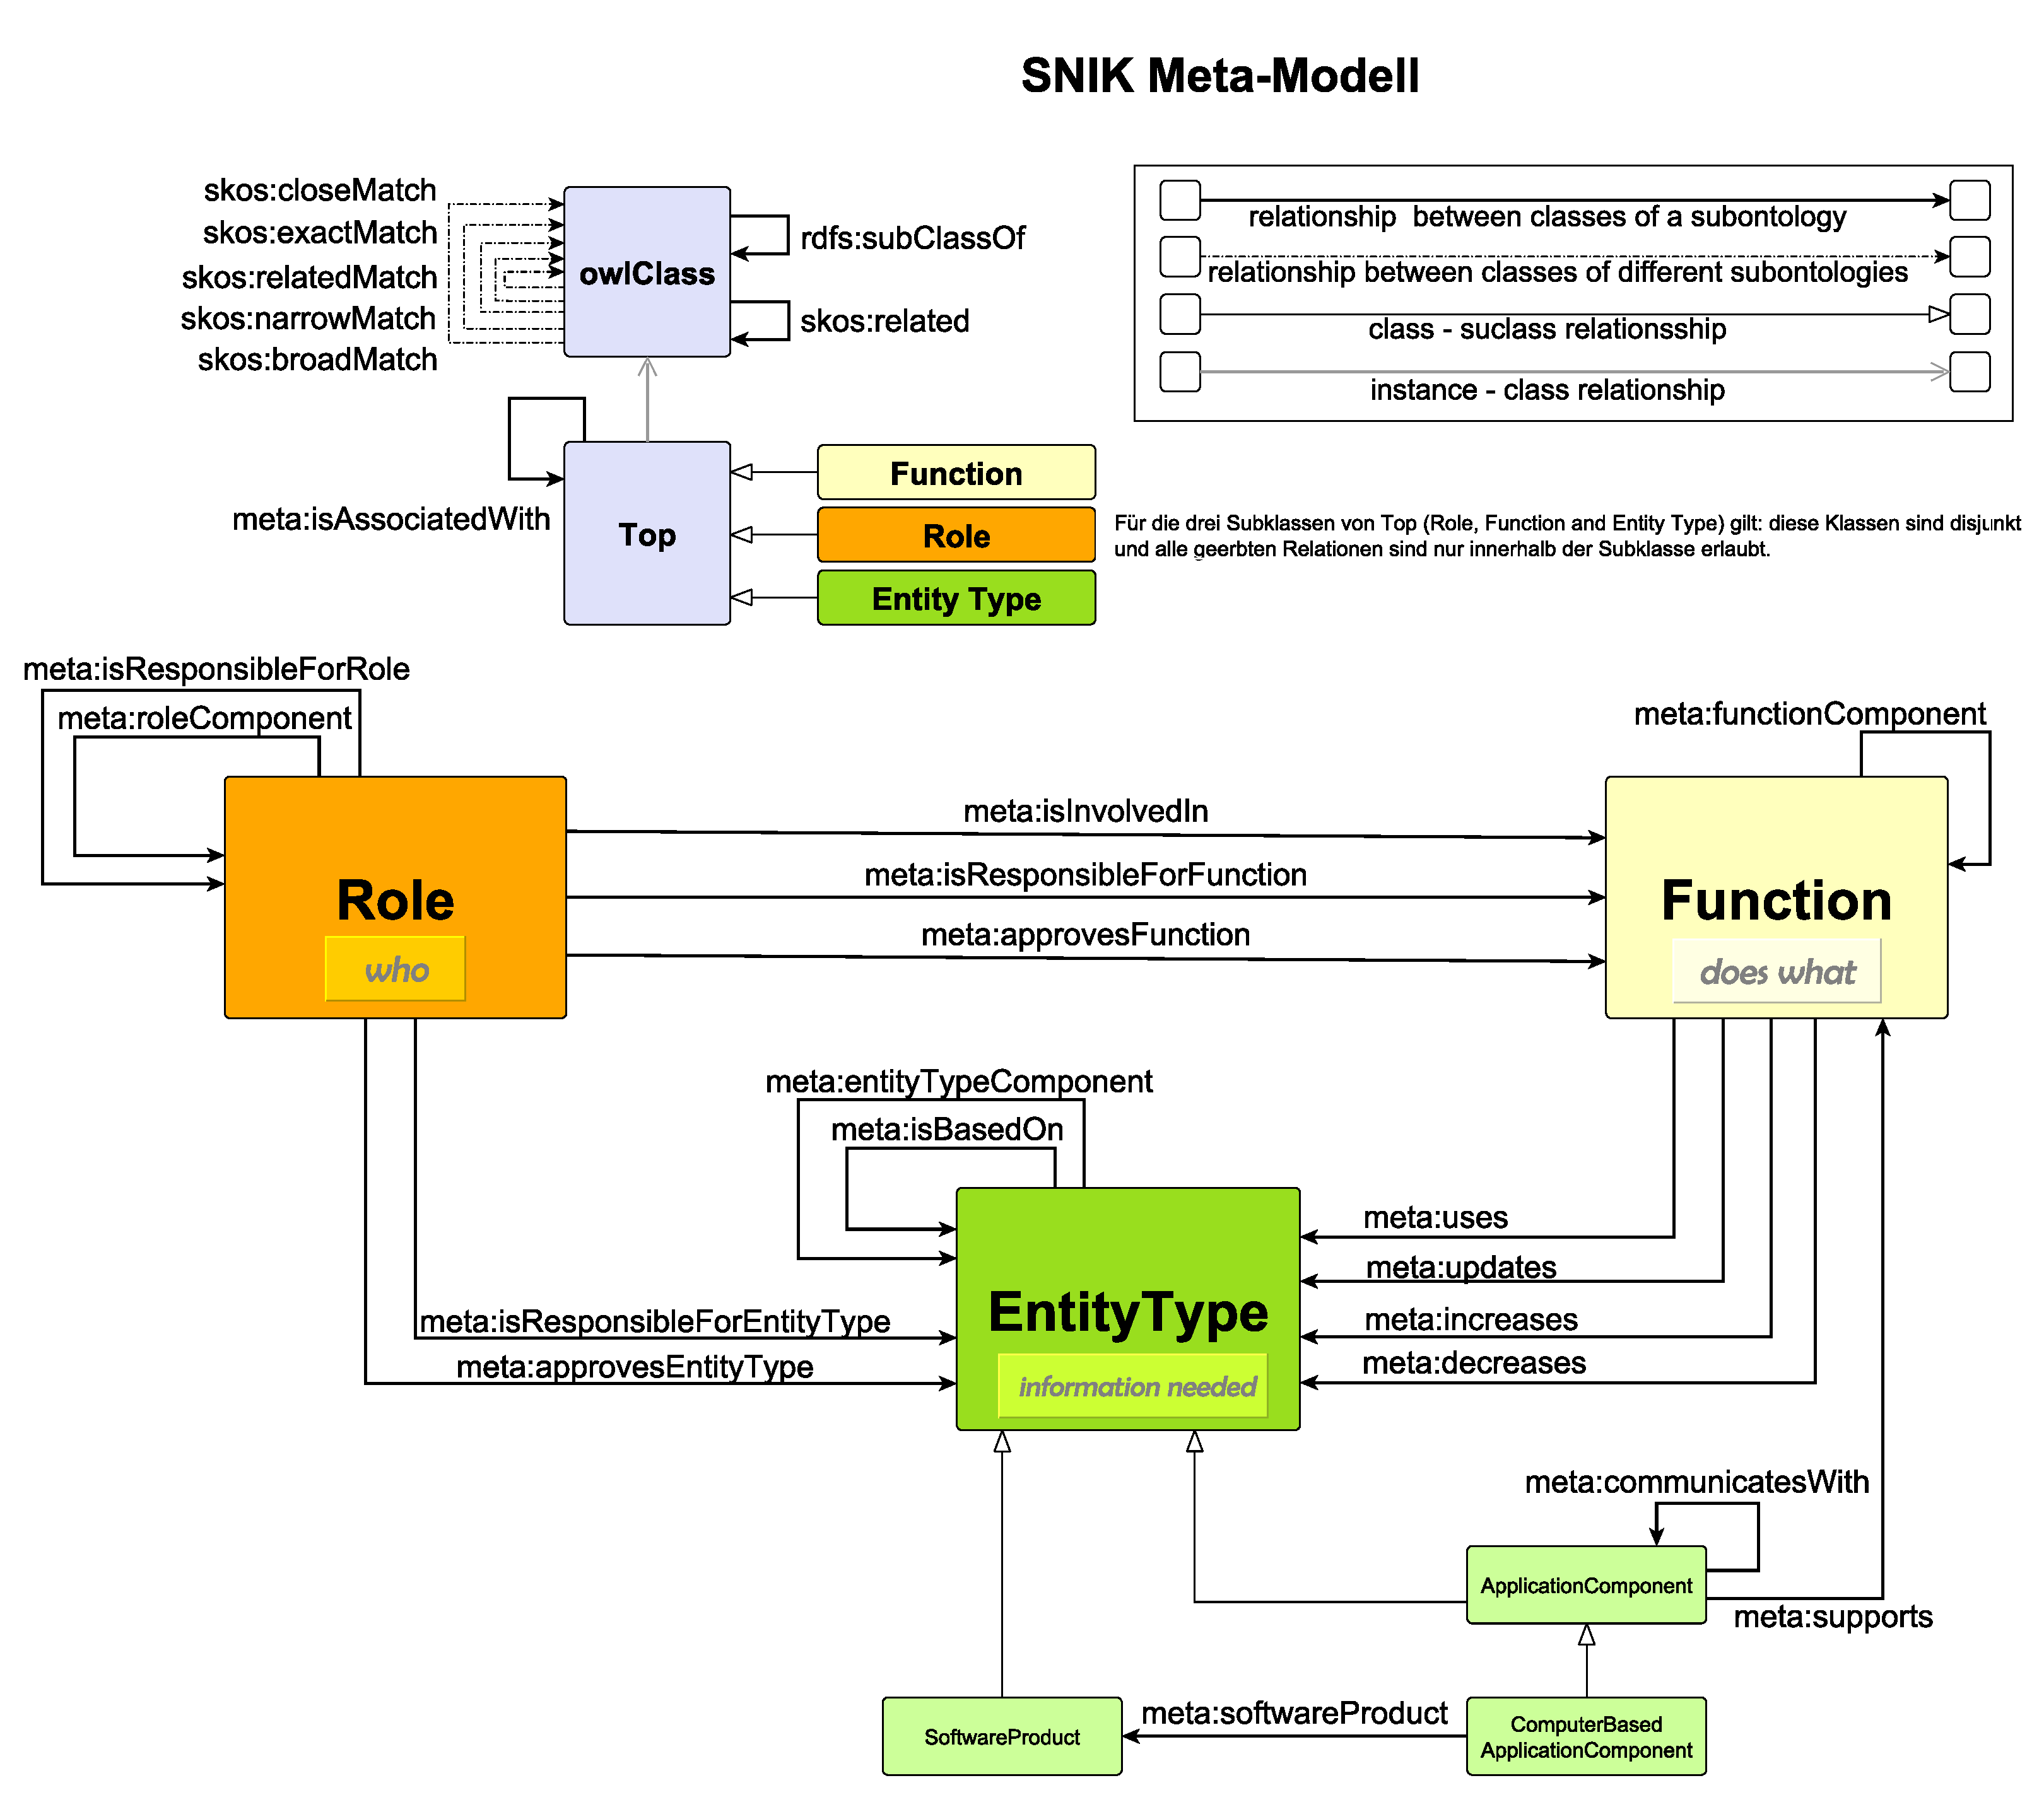
\includegraphics[width=\linewidth]{../Dokumentation/Images/snik-metamodel.pdf}

\end{posterbox}
%%%%%%%%%%%%%%%%%%%%%%%%%%%%%%%%%%%%%%%%%%%%%%%%%%%%%%%%%%%%%%%%%%%%%%%%%%%%%%
\begin{posterbox}[name=methods,below=background]{Methodik}

\end{posterbox}
%%%%%%%%%%%%%%%%%%%%%%%%%%%%%%%%%%%%%%%%%%%%%%%%%%%%%%%%%%%%%%%%%%%%%%%%%%%%%%
\begin{posterbox}[name=results,column=1]{Ergebnisse}
  % PLOTS
  
\end{posterbox}
%%%%%%%%%%%%%%%%%%%%%%%%%%%%%%%%%%%%%%%%%%%%%%%%%%%%%%%%%%%%%%%%%%%%%%%%%%%%%%
\begin{posterbox}[name=discussion,column=1,below=results]{Diskussion}

\end{posterbox}
%%%%%%%%%%%%%%%%%%%%%%%%%%%%%%%%%%%%%%%%%%%%%%%%%%%%%%%%%%%%%%%%%%%%%%%%%%%%%%
\begin{posterbox}[name=references,column=0,below=methods]{Literatur}
    \small
    \begingroup
    \renewcommand{\section}[2]{}%suppress heading
    % using bibtex ***********
    %\bibliographystyle{abbrv}
    %\bibliography{poster}
    % using biblatex *********
    \printbibliography
    %*************************
    \endgroup
    \vspace{0.3em}
    %Myproject is supported under the DFG grant numbers 1234/5-6 and 6543/2-1.
  \end{posterbox}
%%%%%%%%%%%%%%% QAnswer Logo
\node [anchor=south east, inner sep=1pt,xshift=-10em,yshift=7em] at (current page.south east)
{\includegraphics[height=1.5cm]{img/logos/qanswer-logo.png}};
%%%%%%%%%%%%%%% IMISE Logo
\node [anchor=south east, inner sep=1pt,xshift=-3em,yshift=1em] at (current page.south east)
{\includegraphics[height=1.5cm]{img/logos/imise-logo.pdf}};
%%%%%%%%%%%%%%% Medical Faculty Logo
\node [anchor=south east, inner sep=1pt,xshift=-19.5em,yshift=-1.5em] at (current page.south east)
{\includegraphics[height=3.3cm,decodearray=0 0 0 0 0 1]{img/logos/medfak.pdf}};
%%%%%%%%%%%%%%%%%%%%%%%%%%%%%%%%%%%%%%%%%%%%%%%%%%%%%%%%%%%%%%%%%%%%%%%%%%%%%%
\end{poster}
\end{document}

